\chapter{Sviluppo Client}                %crea il capitolo
%%%%%%%%%%%%%%%%%%%%%%%%%%%%%%%%%%%%%%%%%imposta l'intestazione di pagina
\lhead[\fancyplain{}{\bfseries\thepage}]{\fancyplain{}{\bfseries\rightmark}}
\pagenumbering{arabic}                  %mette i numeri arabi

Inizialmente per sviluppare l'applicazione, è stato preso in considerazione il linguaggio Java, successivamente dopo aver testato le funzionalità di Java fu preso in considerazione Kotlin come linguaggio di programmazione per Android, in alternativa a Java.\\
Avendo utilizzato inizialmente Java per scrivere parte del codice dell'applicazione e successivamente riscrivere l'applicazione interamente in Kotlin è stato possibile confrontare concretamente i miglioramenti offerti da Kotlin rispetto a Java.\\
Il Client è stato strutturato in modo da contenere in packages differenti i componenti principali dell'applicazione.
\begin{itemize}
    \item \textbf{Activities:} Contiene le Actvity utilizzate dall'applicazione
    \item \textbf{Pages:} Contiene quattro packages corrispondenti alle 4 funzionalità dell'app
    \item \textbf{Models:} Contiene i modelli, utili per il pattern MVP
    \item \textbf{Repositories:} Contiene classi che facilitano la gestione e le richieste con il database
    \item \textbf{Services:} Contiene due servizi per la gestione delle notifiche
    \item \textbf{Utils:} Contiene classi utili per la gestione della cache, PreferenceShared e Componenti view personalizzati.
\end{itemize}

La struttura e l'organizzazione dei file delle quattro funzionalità dell'app è la stessa, inoltre il pattern utilizzato per la gestione fra le varie componenti del progetto per interagire con i dati e l'interfaccia utente è MVP (Model View Presenter).\\
Esiste una Activity principale chiamato BaseActivity che gestisce il funzionamento dei menù (Menu delle impostazioni, Menù delle funzionalità), e si occupa di mostrare le quattro pagine principali, realizzate estendendo la class Fragment.\\
I quattro Fragment sono quindi:
\begin{itemize}
    \item \textbf{FragmentTodo:} Pagina per visualizzare e interfacciarsi con le faccende del gruppo
    \item \textbf{FragmentSpese:} Pagina per visualizzare e interfacciarsi con le spese del gruppo
    \item \textbf{FragmentEventi:} Pagina per visualizzaere e gestire gli eventi del gruppo
    \item \textbf{FragmentChat:} Pagina per accedere alla chat di messaggistica istantanea del gruppo
\end{itemize}
I fragment vengono cambiati e gestiti dall'Activity principale, che in base all'interazione con il menu delle funzionalità, si interscambiano.
\begin{lstlisting}[language=kotlin,caption={Aggiornamento fragment del BaseActivity}]
 supportFragmentManager.beginTransaction().replace(R.id.activity_content, TodoFragment()).commit()
\end{lstlisting}

Quando si seleziona una della pagine, il controllo dell'interfaccia passa al relativo Fragment, che in base alla funzionalità mostrerà e permetterà di agire sull'interfaccia.\\

\section{Paradigmi e Pattern}
La lagica per gestire l'interazione con l'utente e l'aggiornamento dei dati si basa sul pattern MVP, di conseguenza ogni Fragment o Activity che richiede di mostrare dei dati, implementerà i seguenti componenti:
\begin{itemize}
    \item \textbf{Adapter:} Estensione della classe "RecyclerView.Adapter" che contiene e la lista elementi da visualizzare
    \item  \textbf{Presenter:} Componente che ha il compito di richiedere al Repository i dati da visualizzare
    \item  \textbf{View:} Interfaccia grafica della pagina con cui l'utente può interagire
    \item  \textbf{Model:} Modello astratto da rappresentare nella View
    \item  \textbf{Repository:} Classe che ha il compito di inviare richieste al Database, o di restituire le query necessarie per la richiesta al database
\end{itemize}
\newpage
\subsection{Reactive Programming}
La programmazione reattiva o Reactive Programming è un paradigma di programmazione che monitora e gestisce flussi di dati statici o dinamici e la propagazione dei flussi nel tempo, ciò significa che attraverso dei costrutti messi a disposizione da librerie che implementano il concetto di programmazione reattiva sarà possibile sviluppare applicazioni basate sugli eventi.\\
Il concetto fondamentale utilizzato in questo paradigma è la possibilità di creare flussi di qualsiasi tipo sia facendo riferimento al click dell'utente sull'interfaccia grafica sia a variabili, input utente, proprietà, cache, strutture dati e richieste HTTP.\\
Un flusso è una sequenza di eventi ordinati nel tempo che può emettere tre risposte differenti: un valore (di qualche tipo), un errore o un segnale per indicare che il flusso è terminato. Questi tre eventi vengono gestiti in modo asincrono, definendo una funzione che verrà eseguita quando viene emesso un valore, un'altra funzione quando viene emesso un errore e un'altra funzione quando viene completato il flusso.\\
I due componenti principali sono quindi ``Observables'' ovvero colui che emette un flusso di dati
e ``Observers'', ovvero colui che monitora il flusso e rimane in ascolto di nuovi valori.

\begin{figure}[!hb]
  \centering
  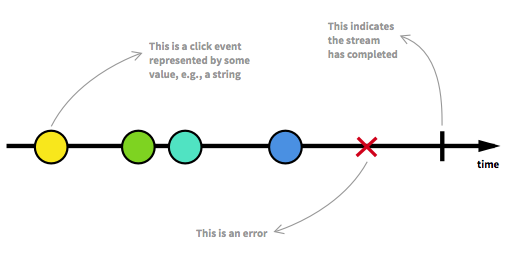
\includegraphics[width=0.65\textwidth]{immagini/reactive_programming_es1.png}
  \caption{Reactive Programming Esempio 1}\label{fig:Reactive Programming Esempio 1}
\end{figure}

\newpage
\begin{itemize}
  \item \textbf{onNext}: Metodo che viene richiamato quando un Observable emette  un  nuovo elemento nel corso del flusso
  \item  \textbf{OnComplete:} Metodo che indica che il flusso è giunto al termine e quindi non verrà emesso nessun nuovo elemento
  \item \textbf{onError} Metodo che viene chiamato in presenza di errori all'interno del flusso, questo metodo interrompe il normale percorso del flusso.
\end{itemize}

Nello sviluppo dell'applicazione è stata utilizzata la libreria RxJava per utilizzare il paradigma di programmazione reattiva, e sfruttare la logica e i benefici della programmazione asincrona.\\
In particolare la libreria è stata utilizzata per la gestione dei flussi di dati durante le richieste effettuate al database Firestore.

\begin{figure}[!hb]
  \centering
  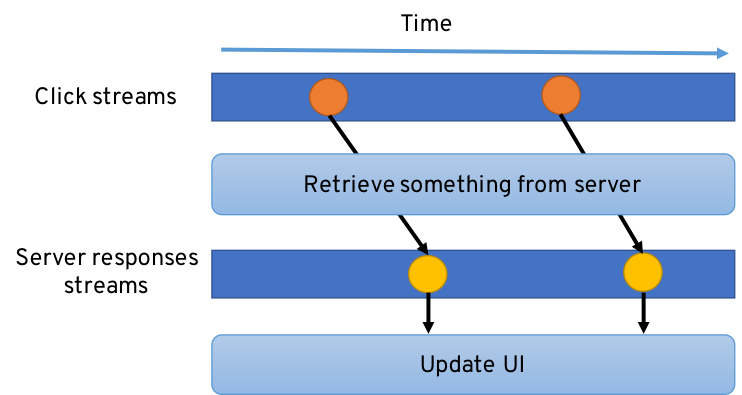
\includegraphics[width=1\textwidth]{immagini/reactive_programming_es2.png}
  \caption{Reactive Programming Esempio 2}\label{fig:Reactive Programming Esempio 2}
\end{figure}
Quando un utente si interfacciava con la pagina di una funzionalità veniva effettuata la richiesta al server e aggiornata l'interfaccia con i nuovi dati.
\newpage



\subsection{Repository}
All'interno del package Repositories sono presenti le classi necessarie per interagire con il database Firestore.\\
Sono presenti due tipi di classi:
\begin{itemize}
    \item \textbf{Query:} Sono classi che contengono le query necessarie per interagire con il database, ogni classe conterrà le query relativa alle sue funzionalità, la funzione Todolist dell'applicazione ad esempio avrà una classe TodoListQuery.
    \item \textbf{Repository:} Sono classi che restituiscono un oggetto Single, Observable o Completable in base al tipo di richiesta effettuata. Ogni Repository richiamerà la relativa classe Query per ricevere l'istruzione necessaria per aggiungere modificare o richiedere dei dati al database.
\end{itemize}

Un esempio di una Repository è il seguente:

\begin{lstlisting}[language=kotlin,caption={Esempio RepositoryAggiunta elemento Todolist}]
fun getTodoItems(): Single<List<TodoItem>> {
       return Single.create<List<TodoItem>> { emitter ->
           queryTodo.getTodoItems().addSnapshotListener({ querySnapshot, exception ->
               if (exception != null)
                   emitter.onError(Throwable(exception))
               else {
                   emitter.onSuccess(TodoItem.mapping(querySnapshot))
               }
           })
       }
   }
\end{lstlisting}
Ogni Repository non conosce la query necessaria per effettuare la richiesta al database ma utilizzando la rispettiva classe che restituisce la query necessaria per richiedere al database la lista degli elementi all'interno della todolist.



\subsection{Utils}
Il package Utils contiene classi di supporto per azioni comuni che vengono svolte dai componenti dell'applicazione.\\
In particolare le principali sono:
\begin{itemize}
    \item \textbf{PreferenceUtils:} Classe utilizzata per gestire le SharedPreferences
    \item \textbf{ImageUtils:} Classe che interagendo con la libreria Glide, aggiunge funzionalità alla gestione delle immagini
    \item \textbf{RxFirestore:} Estensioni effettuate su alcuni oggetti dell'SDK Firestore per implementare il pattern Observable
    \item \textbf{UserSpinner:} Componente View che estende AppCompatSpinner, creato per mostrare e selezionare graficamente gli utenti attraverso uno spinner
    \item \textbf{FirestoreCMUtils:} Classe che gestire i Token utilizzati da Cloud Messaging
\end{itemize}

La classe PreferenceUtils memorizza le informazioni riguardanti gli utenti apparteneti al gruppo, le informazioni personali dell'utente consentendo di modificarne i valori e cancellare tutti i dati e le cache dell'applicazione.\\.
La classe ImageUtils, è stata realizzata per estendere alcune funzionalità della libreria Glide, utilizzata per visualizzare le immagini, in particolare è stato implementato un metodo per visualizzare un immagine attraverso un link URL. La libreria opportunamente mofiticata consetiva successivamente di scaricherà l'immagine, memorizzarla nella cache e renderla visibile all'utente nell'interfaccia.\\
Il file RxFirestore contiene le funzioni necessarie per implementare dei metodi aggiuntivi agli oggetti DocumentReference, CollectionReference messi a disposizione dall'SDK di Firebase per fare riferimento ad una collezzione o documento all'interno del database. I metodi aggiuntivi consentono di applicare la programmazione reattiva alle chiamate eseguite per richiedere e modificare dati all'interno del database Firestore.
UserSpinner è un widget creato appositamente per mostrare una finestra di dialogo contenente la lista del nome degli utenti appartenenti al gruppo, e una checkbox per ogni utente, offrendo quindi la possibilità di selezionare uno o più utenti durante la creazione di una nuova faccenda, spesa o evento.\\
Infine la classe FirestoreCMUtils gestisce i token e i gruppi associati ad un token di Cloud Messaging, la classe in particolare viene utilizzata per generare un token necessario per connettersi ai server FCM, creare un nuovo gruppo di utenti indicando i token di ogni dispositivo, e per ultimo gestire l'aggiunta di un nuovo utente ad un gruppo di utenti preesistenti.

\subsection{Modelli}
I modelli sono stati realizzati utilizzando le data class offerte da Kotlin, in questo modo non è stato necessario implementare i metodi get e set come quando si devono creare dei modelli in Java. L'unica aggiunta effettuata è stata la creazione di due nuovi metodi chiamati "mapping" che permettono di convertire i tipi DocumentSnapshot e QuerySnapshot restituiti dal'SDK Firebase come risposta ad una richiesta effettuata al database Firestore in modelli utilizzabili come oggetti all'interno dell'applicazione, mappando quindi ogni valore contenuto negli SnapShot all'interno dei singoli valori del modello.\\
I modelli vengono utilizzati nell'applicazione per rispettare il pattern MPV garantendo una buona interazione dei dati con l'interfaccia grafica, e soprattutto per avere una migliore gestione dei tipi durante la chiamata e la restituzione di valori associati ad una funzione.\\
Un esempio di un modello utilizzato è il seguente:
\begin{lstlisting}[language=kotlin,caption={Aggiunta elemento Todolist}]

data class GroupItem(
        var id: String = "",
        var name: String? = null,
        var creation_date: Date = Date(),
        var logo: String? = null,
        var users: Map<String, Boolean> = emptyMap(),
        var tokenFCM: String? = null
)
\end{lstlisting}
Il seguente modello rappresenta un documento all'interno della collezzione contenente i gruppi. Attraverso il costrutto data class, e inizializzando le variabili con la keyword "var" Kotlin in automatico in fase di compilazione aggiungerà i metodo necessari per settare e ricevere i valori dalla classe GroupItem.\\
L'id di ogni gruppo è impostato a stringa vuota, e verrà settato al momento dell'aggiunta di un nuovo gruppo, come il nome il logo e la lista degli utenti.\\
Il valore data è assegnato di default in base alla data di creazione del gruppo, mentre il tokenFCM è generato subito dopo la creazione del gruppo, attraverso il servizio FCM.

\subsection{Servizi}
I servizi utilizzati dall'applicazione sono stati creati per interagire con il servizio Cloud Messaging di Firebase.\\
I servizi sono due:
\begin{itemize}
    \item \textbf{FirebaseMessagingService}
    \item \textbf{FirebaseInstanceIdService}
\end{itemize}

Il primo: FirebaseMessagingIdService gestisce i token necessari per utilizzare Cloud Messaging, in particolare gestisce l'aggiornamento del token del dispositivo, inviando una richiesta di aggiornamento al Database Firestore, qualosa il token sia aggiornato o eliminato.\\
Il secondo servizio invece: FirebaseInstanceService gestisce i messaggi ricevuto dal server di Cloud Messaging, implementando il metodo onMessageReceived sarà possibile innanzitutto capire il tipo di messaggio ricevuto da FCM (messaggio di notifica o messaggio contenente dati), successivamente in base al tipo di messaggio ricevuto vengono effettuate modifiche o mostrate le adeguate notifiche.\\
Oltre ad aggiungere la libreria che si occupa di interagire con il servizio FCM, è stato necessario indicare all'interno del AndroidManifest del progetto, che le due classi create sono dei servizi:
\begin{lstlisting}[language=kotlin,caption={Android Manifest - I servizi FCM}]

<service android:name=".Services.FirestoreEventFunctionService">
           <intent-filter>
               <action android:name="com.google.firebase.MESSAGING_EVENT" />
           </intent-filter>
       </service>

       <service android:name=".Services.FirestoreEventFunctionnstanceIDService">
           <intent-filter>
               <action android:name="com.google.firebase.INSTANCE_ID_EVENT" />
           </intent-filter>
       </service>

       \end{lstlisting}
In particolare quando viene ricevuto il messaggio di aggiunta di un nuovo membro nel gruppo, oltre ad inviare la notifica per avvisare i dispositivi, vengono anche aggiornate le PreferenceShared che contiene localmente una copia delle informazioni riguardanti il gruppo senza dover contattare ogni votla il database.\\

\begin{lstlisting}[language=kotlin,caption={Metodo onMessageReceived}]

override fun onMessageReceived(remoteMessage: RemoteMessage ? ) {
...
  val msgData = remoteMessage.data.toProperties()
  val loggedUser = PreferenceUtils(context = applicationContext).getUserUID()
  if (remoteMessage.data.isNotEmpty()) {
   val msgData = remoteMessage.data.toProperties()
   val loggedUser = PreferenceUtils(context = applicationContext).getUserUID()
   if (msgData.getProperty("sender") != loggedUser) {
    when(msgData.getProperty("type")) {
      ...
     "todo" -> {
      sendNotification(messageTitle = R.String.new_todo_item, messageBody = msgData.getProperty("name"))
     }
     ...
    }
   }
  }
}
\end{lstlisting}
La funzione "onMessageReceived" viene richiamata quando il server FCM segnala al dispositivo la ricezione di un nuovo messaggio. Successivamente, verrà controllato se l'utente che ha compiuto il cambiamento all'interno del database, aggiungendo o modificando un elemento, è lo stesso utente loggato all'interno dell'applicazione, in caso affermativo non verrà inviata nessuna notifica al dispositivo, in caso constrario verrà mostrata una notifica, avvisando l'utente del nuovo cambiamento all'interno dell'applicazione.

\subsection{Todolist e Spese}
Le due pagine pur avendo funzionalità differenti hanno un interfaccia e logica molto simile di conseguenza verra presa in considerazione solamente la pagina delle faccende.\\
Il fragment TodolistPage, si occupa di gestire l'aggiunta rapida di un nuovo elemento e la logica delle due Tab "Da completare" "Completato".\\
L'aggiunta di un elemento con la modalità rapida, inserendo solamente il nome della faccenda, viene svolta, inizializza un nuovo elemento di tipo Todolist, contenente il nome inserito dall'utente e impostando i valori di default della faccenda.\\ Successivamente viene inizilizzata la Repository che ha il compito di gestire l'interazione con il database per la lista delle faccende. attraverso un approccio asincrono, il fragment attenderà la risposta dal Database e in caso negativo mostrerà un errore.

\begin{lstlisting}[language=kotlin,caption={Aggiunta elemento Todolist}]
val todoItem = TodoItem(name = itemName, date = Date(), members = members, created_by = userUID)
todoRepo.add(todoitem = todoItem).observeOn(AndroidSchedulers.mainThread()).subscribeOn(Schedulers.io()).doOnComplete {
    todolist_editext_newitem.setText("")
    Toast.makeText(context, "todoitem successfully created!", Toast.LENGTH_SHORT).show()
}.doOnError {
            Toast.makeText(context, "error!", Toast.LENGTH_SHORT).show()
        }.subscribe()
\end{lstlisting}

Il componente TabLayout che mostra le due Tab richiede l'utilizzo di un Adapter che estende la class FragmentStatePagerAdapter, in questo modo quando un utente interagirà con una delle due Tab, l'Adapter si occuperà di istanziare il Fragment corrispondente per visualizzare la lista delle faccende completate o non completate.\\
Dato che per visualizzare gli elementi completati e da completare, teoricamente sarebbero servite due Fragment con parti di codice molto simile, si è scelto di realizzarene solamente uno, che in base al valore di un parametro chiamato ``type'' passato nella creazione dell'istanza del fragment, visualizzerà elementi differenti.\\

\begin{lstlisting}[language=kotlin,caption={FragmentTodo.kt}]
companion object {
       fun newInstance(type: Int): TodoFragment {
           val fragment = TodoFragment()
           fragment.type = type
           return fragment
       }
   }
\end{lstlisting}


\subsection{Eventi}
Gli utenti hanno la possibilità di aggiungere all'interno del gruppo eventi classici ed eventi ricorrenti. La logica utilizzata per visualizzare ed aggiungere elementi all'interno del database è la stessa utilizzata per le precedenti funzionalità, è quindi presente un fragment principale, una view, un presenter che richiede al database firestore i dati da visualizzare, e un adapter.\\
Durante l'aggiunta di un nuovo elemento è stata usata la libreria SublimePicker che offre l'interefacia di un calendario personalizzabile, con cui far interagire l'utente per selezionare una data e impostare una ricorrenza. Il Widget SublimePicker necessita di un inizializzazione con il passaggio di un oggetto ``SublimeOptions'' per poter funzionare.\\

\begin{lstlisting}[language=kotlin,caption={Configurazione del Widget SublimePicker}]
..
val options = SublimeOptions()
var displayOptions = 0
displayOptions = displayOptions or SublimeOptions.ACTIVATE_DATE_PICKER
displayOptions = displayOptions or SublimeOptions.ACTIVATE_RECURRENCE_PICKER
options.pickerToShow = SublimeOptions.Picker.REPEAT_OPTION_PICKER
options.setDisplayOptions(displayOptions)
options.setCanPickDateRange(false)
..

\end{lstlisting}
Una volta indicati i parametri di default del Widget sarà possibile renderlo disponibile graficamente all'utente.
Nella visualizzazione degli eventi per distingue se un evento è ricorrente è stato ricavato un nuovo dato non presente nel database, che consiste nel differenziare eventi ricorrenti da eventi che non hanno nessuna ricorrenza.\\

\begin{lstlisting}[language=kotlin,caption={Linea di codice del modello Event}]
   var is_recurring = result.getString("recurring_type").isNullOrBlank().not()
\end{lstlisting}

Gli eventi ricorrenti hanno assegnato il valore di ricorrenza (Dayly,Weekly,Monthly,Yearly) all'interno della variabile ``recurring'\_type'', di conseguenza effettuando un controllo sul contenuto della variabile è possibile creare la variabile booleana ``is'\_Recurring'' che differenzia i due tipi di eventi

\newpage

\subsection{Chat}
La chat come le precedenti pagine, utilizza il pattern MVP, di conseguenza all'iterno del fragment verranno instanziati il Presenter l'Adapter e implementata la View.\\
La chat per facilitare la visione dei messaggi ricevuti e inviati all'iterno dell'Adapter prevede due differenti ViewHolder che differenziano il messaggio inviato da quello ricevuto.\\
La realizzazione di questa distizione grafica fra i due tipi di messaggio inizialmente è stata creata una classe astratta ChatHolder che avesse come unico metodo la funzione "bind" e prendesse come parametro il messaggio, in modo tale che i due holder verranno implementati basandosi e estendendo questa classe.\\
Successivamente sono state sovrascritti i metodi getItemViewType e onCreateViewHolder del Fragment in modo tale da introdurre il controllo necessario per distinguere i messaggi.\\
All'interno del metodo getItemViewType, viene controllato il campo "SenderUID" del messaggio, corrispondente all'ID dell'utente che ha inviato il messaggio nel gruppo, questo ID viene poi confrontato con l'ID dell'utente loggato all'interno dell'applicazione in modo da restituire l'identificativo del layout da utilizzare nel ViewHolder.
\begin{lstlisting}[language=kotlin,caption={Logica della funzione getItemViewType della Chat}]
when (senderUid == userUid) {
    false -> return R.layout.item_message_recived
    true -> return R.layout.item_message_sent
}
\end{lstlisting}
Una volta differenziato il tipo attraverso il metodo getItemViewType, è stata sovrascritto il metodo onCreateViewHolder che dovendo restituire un singolo Holder, come valore di ritorno restituisce un tipo ChatHolder (classe astratta implementata dalle due ViewHolder). In questo modo in base al tipo restituito da getItemViewType la classe onCreateViewHolder restituirà l'holder corrispondente al messaggio.
\begin{lstlisting}[language=kotlin,caption={Logica della funzione onCreateViewHolder della chat}]

when (viewType) {
           R.layout.item_message_sent -> holder = MessageChatSentHolder(itemView = view, dateOfLastMessage = lastItem?.timestamp)
           R.layout.item_message_recived -> holder = MessageChatRecivedHolder(itemView = view, dateOfLastMessage = lastItem?.timestamp)
       }
   \end{lstlisting}



\subsection{Librerie}
Il progetto è stato realizzato utilizzando librerie open source importante e gestite da Gradle, un programma per l'automazione dello sviluppo.\\
Gradle è stato progettato per automatizzare il processo di generazione di un progetto, facilitando l'aggiunta di librerie esterne, la compilazione finale del progetto comprese le sue dipendenze e l'aggiunta di test automatizzati.\\
La lista delle librerie utilizzate nel progetto possono essere divise in quattro categorie:
\begin{itemize}
    \item Librerie di supporto per Android e Kotlin
    \item Librerie SDK di Firebase
    \item Libreria per il supporto della programmazione reattiva
    \item Librerie per la gestione delle immagini
    \item Librerie per componenti grafici aggiuntivi
\end{itemize}

\newpage
Le librerie offerte da Android per il supporto di funzionalità e componenti grafici aggiuntivi sono le seguenti:
\begin{table}[!h]
\begin{center}
\begin{tabular}{|l|p{7cm}|}
    \hline
\textbf{Libreria} & \textbf{Descrizione}\\ \hline
com.android.support:support & Libreria di supporto per Android  \\ \hline
com.android.support:appcompat & Supporto per i componenti grafici aggiuntivi \\ \hline
com.android.support:recyclerview & Widget personalizzabile simile al ListView ma più avanzato e flessibile \\ \hline
com.android.support:cardview & Componente per realizzare interfacce Material Design \\ \hline
com.android.support:design & Libreria di supporto per l'interfaccia Android  \\ \hline
com.android.support:constraint-layout & Layout personalizzabile \\ \hline
com.google.android:flexbox  & Layout personalizzabile Flex per Android  \\ \hline
com.android.support:customtabs & Libreria di supporto per il widget Tab  \\ \hline
android.arch.lifecycle:extensions & Supporto per Android Components Architecture \\ \hline
com.android.support:vector-drawable & Supporto per immagini svg e vettoriali  \\ \hline
android.arch.lifecycle:common-java8 &  Supporto per la gestone del lifecycle Android \\ \hline
org.jetbrains.kotlin:kotlin-stdlib-jre7 & Supporto per il linguaggio Kotlin su Android \\ \hline
\end{tabular}
\caption[Librerie Google del progetto]{Librerie Google del progetto}\label{tab:Librerie Google del progetto}
\end{center}
\end{table}

\newpage

Le librerie di supporto offerte da Firebase per utilizzare i suoi servizi sono le seguenti:

\begin{table}[!h]
\begin{center}
\begin{tabular}{|l|p{7cm}|}
    \hline
\textbf{Libreria} & \textbf{Descrizione}\\ \hline
com.google.android.gms:play-services-auth  & Libreria di supporto per i servizi Google  \\ \hline
com.google.firebase:firebase-auth & SDK del servizio di autenticazione di Firebase \\ \hline
com.google.firebase:firebase-firestore & SDK per interfacciarsi con il database Firestore \\ \hline
com.google.firebase:firebase-storage & SDK per usufruire dello storage di Firebase  \\ \hline
com.google.firebase:firebase-messaging & SDK del servizio di messaggistica \\ \hline
com.firebase:firebase-jobdispatcher  & Supporto per lo scheduling e l'esecuzione in background\\ \hline
com.firebaseui:firebase-ui-auth & Libreria di supporto per il servizio Firebase-Auth  \\ \hline
com.firebaseui:firebase-ui-firestore & Libreria di supporto per il servizio Firestore  \\ \hline
com.firebaseui:firebase-ui-storage & Libreria di supporto per il servizio Storage  \\ \hline
com.facebook.android:facebook-android-sdk & SDK per l'accesso tramite il social Facebook \\ \hline
com.twitter.sdk.android:twitter-core & SDK per l'accesso tramite il social Twitter \\ \hline
\end{tabular}
\caption[Librerie Firebase del progetto]{Librerie Firebase del progetto}\label{tab:Librerie Firebase del progetto}
\end{center}
\end{table}

\newpage


Le librerie di supporto per implementare la programmazione reattiva sono i seguenti:


\begin{table}[!h]
\begin{center}
\begin{tabular}{|l|p{8cm}|}
    \hline
\textbf{Libreria} & \textbf{Descrizione}\\ \hline
io.reactivex.rxjava2:rxjava:& Supporto dei costrutti della programmazione reattiva su Java  \\ \hline
io.reactivex.rxjava2:rxkotlin & Supporto per la programmazione reattiva su Kotlin  \\ \hline
io.reactivex.rxjava2:rxandroid & Supporto della libreria RxJava2 su Android  \\ \hline
\end{tabular}
\caption[Librerie di supporto per il Reactive programming]{Librerie di supporto per il Reactive programming}\label{tab:Librerie di supporto per il Reactive programming}
\end{center}
\end{table}

Infine le librerie che offrono componenti grafici aggiuntivi sono le seguenti:
\begin{table}[!hb]
\begin{center}
\begin{tabular}{|l|p{7cm}|}
    \hline
\textbf{Libreria} & \textbf{Descrizione}\\ \hline
com.github.ittianyu:BottomNavigationViewEx  & Widget per il menu di navigazione  \\ \hline
com.stephentuso:welcome  & Libreria per mostrare pagine di presentazione e introduzione iniziali \\ \hline
com.shuhart.moneyedittext:moneyedittext-kotlin  & Widget per indicare l'ammontare di una spesa \\ \hline
br.com.simplepass:loading-button-android  & Widget che trasforma un Button in unna barra di caricamento  \\ \hline
com.github.Mariovc:ImagePicker  & Libreria di supporto per selezionare un'immagine dalla galleria del dispositivo  \\ \hline
com.github.bumptech.glide:glide & Libreria per la gestione delle immagini con funzionalità di caching \\ \hline
de.hdodenhof:circleimageview  & Libreria per visualizzare immagini con un bordo circolare \\ \hline
com.appeaser.sublimepickerlibrary:sublimepickerlibrary & Libreria per la selezione di una data dal calendario personalizzabile  \\ \hline
\end{tabular}
\caption[Librerie Firebase del progetto]{Librerie Firebase del progetto}\label{tab:Librerie Firebase del progetto}
\end{center}
\end{table}
